\documentclass[a4paper]{article}
\usepackage{tikz}
\usepackage[margin=.5cm]{geometry}

\begin{document}
    \thispagestyle{empty}
    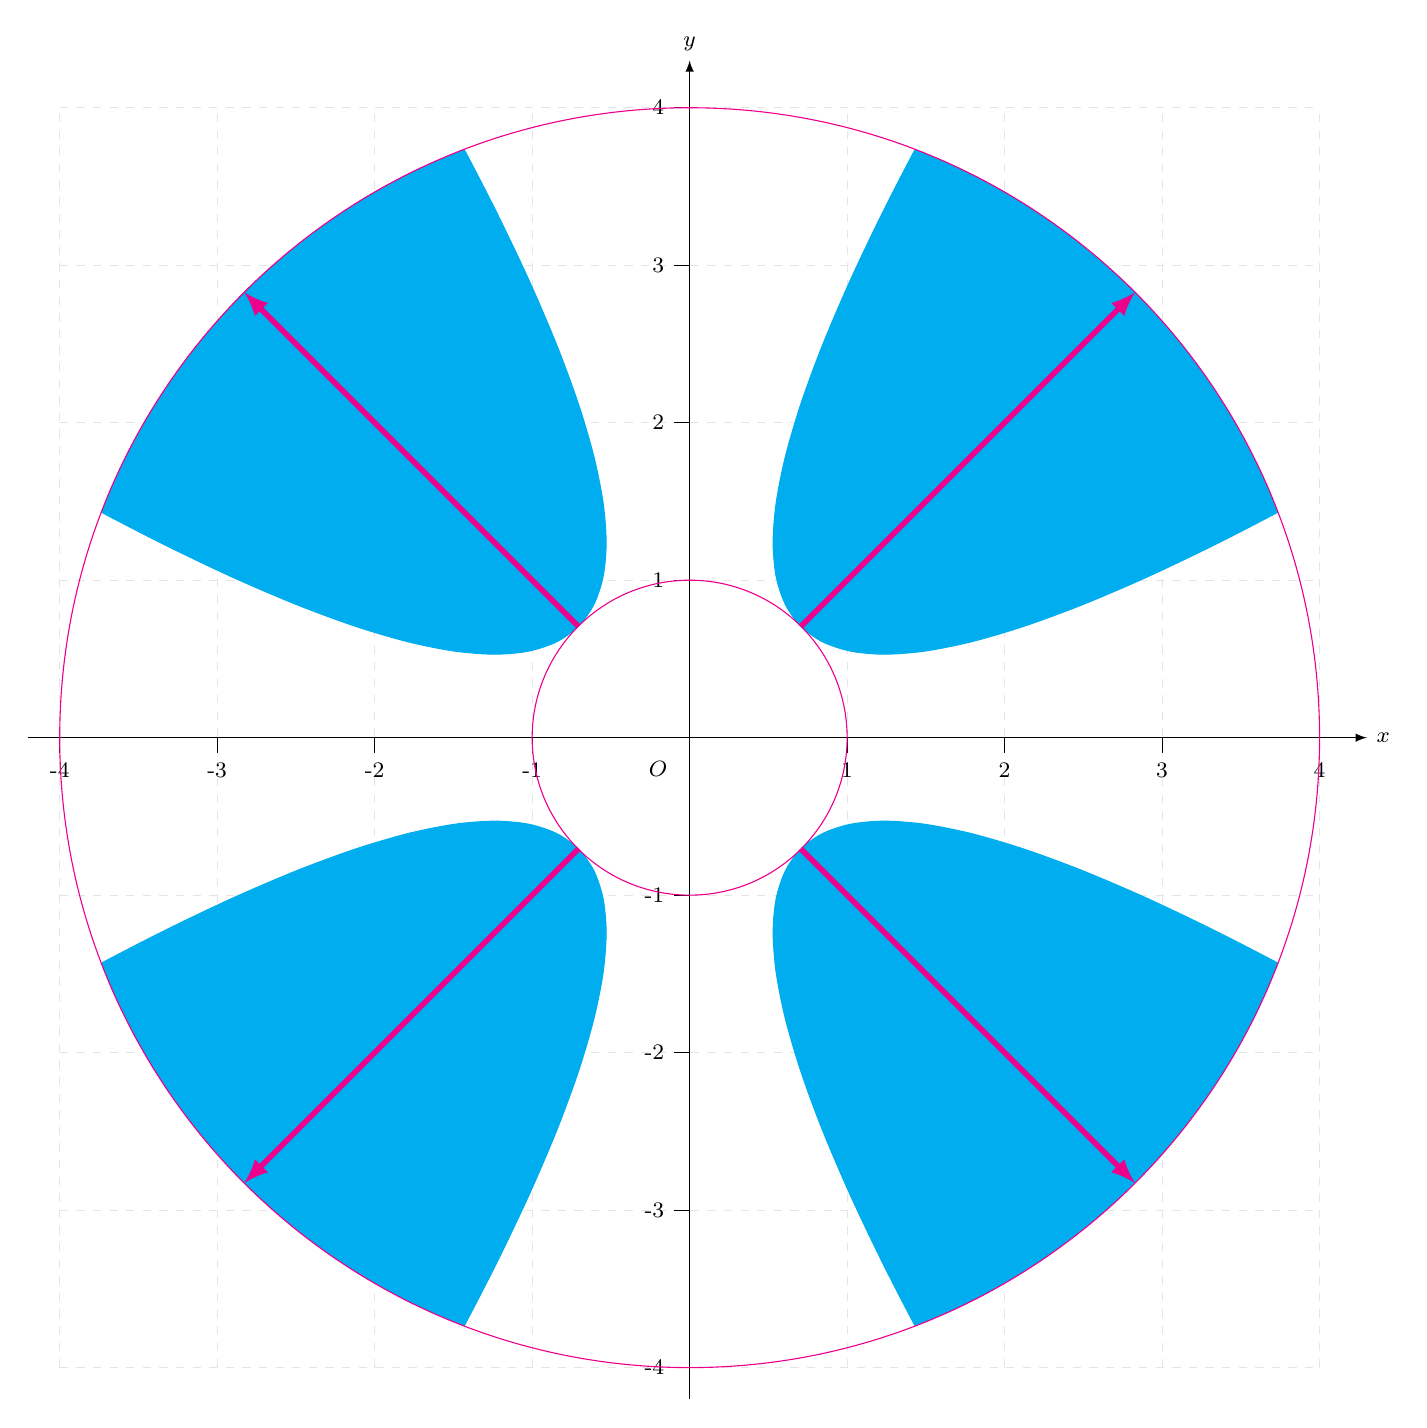
\begin{tikzpicture}[scale=2]
        \draw[gray!20,dashed] (-4,-4) grid (4,4);
        \draw[-latex] (-4.2,0)--(4.3,0) node[right] () {\footnotesize $x$};
        \foreach \i in {-4,...,-1,1,2,...,4}
            \draw (\i,-0)--(\i,-0.1) node[below] () {\footnotesize \i};
        \draw[-latex] (0,-4.2)--(0,4.3) node[above] () {\footnotesize $y$};
        \foreach \i in {-4,...,-1,1,2,...,4}
            \draw (0,\i)--(-.1,\i) node[left] () {\footnotesize \i};
        \draw (-.2,-.2) node () {\footnotesize $O$};
        \begin{scope}
            \clip (0,0) circle(4);
            \foreach \a in {45,135,225,315}{
            \draw[cyan,fill] plot[domain=-2:2,smooth,rotate=-90+\a] (\x,{\x*\x+1});
            \draw[-latex,magenta,line width=2pt,rotate=\a] (1,0)--(4,0);
            }
        \end{scope}
        \draw[magenta] (0,0) circle(1);
        \draw[magenta] (0,0) circle(4);
        
    \end{tikzpicture}

    \end{document}